\section{The Fourier and Wavelet Transforms}

  Computer vision is an extremely difficult task. Pixel intensities in an image are
  typically not very informative in understanding what is in that image. Indeed,
  these values are sensitive to lighting conditions and camera configurations.
  It would be easy to take two photos of the same scene and get two vectors
  $x_1$ and $x_2$ that have a very large Euclidean distance, but to a human,
  would represent the same objects. What is most important in defining an image is
  difficult to define, however some things are notably more important than
  others. In particular, the location or phase of the waves that make up an
  image is much more important than the magnitude of these waves, something
  that is not necessarily true for audio processing. A simple experiment to
  demonstrate this is shown in \autoref{fig:ch2:barbara_morph}. 
  \begin{figure}
    \centering
      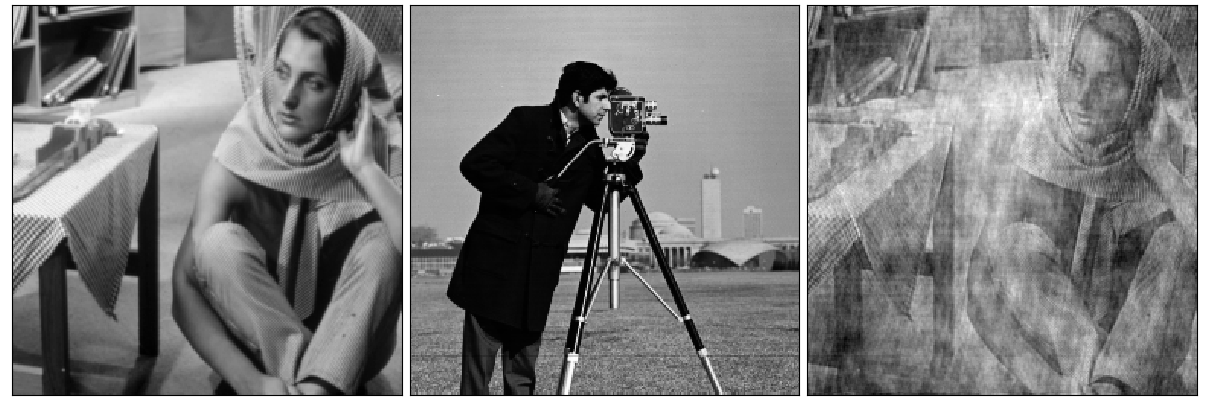
\includegraphics[width=\textwidth]{\imgpath/barbara_mag_swap.png}
      \mycaption{Importance of phase over magnitude for images}
        {The phase of the Fourier transform of the first image is combined with
        the magnitude of the Fourier transform of the second image and
        reconstructed. Note that the first image has entirely won out and
        nothing is left visible of the cameraman.}
      \label{fig:ch2:barbara_morph}
  \end{figure}

\subsection{The Fourier Transform}
For a signal $f(t) \in L_2(\reals)$ (square summable signals), the \emph{Fourier
transform} is defined as:
\begin{equation}
  F(\omega) = \int_{-\infty}^{\infty} f(t) e^{-j\omega t} dt
\end{equation}
This can be extended to two dimensions for signals $f(\xy) \in L_2(\reals[2])$:
\begin{equation}
  F(\ww) = \int_{-\infty}^{\infty}\int_{-\infty}^{\infty} f(\xy) e^{-j\ww^t \xy} d\xy = \langle f(\xy),\ e^{j\ww^t \xy} \rangle
\end{equation}

The Fourier transform is an invaluable signal expansion, as viewing a signal in
the frequency space offers many insights, as well as affording many very useful
properties (most notably the efficiency of convolution as a product of Fourier
transforms). While it is a mainstay in signal processing, 
it can be a poor
feature descriptor due to the infinite support of its basis functions - the
complex sinusoids $e^{j\ww^t u}$. If
a single pixel changes in the input it can change all of the
Fourier coefficients. As natural images are generally non-stationary, we need
to be able to isolate frequency components in local regions of an image, and
not have this property of global dependence.

% The Fourier transform does have one nice property, however, in that the magnitude of
% Fourier coefficients are invariant to global translations, a nuisance
% variability. We explore this theme more in our review of the Scattering
% Transform by \Mallat in \autoref{ch:scatternets}.

\subsection{The Continuous Wavelet Transform}
The \emph{Continuous Wavelet Transform} (CWT), like the Fourier Transform, can be used
to decompose a signal into its frequency components. Unlike the Fourier
transform, these frequency components can be localized in space. To
achieve this, we need a bandpass filter, or \emph{mother wavelet} $\psi$ such that:
\begin{equation}
  \int_{-\infty}^{\infty} \psi(\xy) d\xy = \Psi(0) = 0\label{eq:ch2:admissibility}
\end{equation}
Any function that sufficient decay in frequency and satisfies
\eqref{eq:ch2:admissibility} satisfies the \emph{admissibility condition}.

As we are working in 2-D for image processing, consider dilations, shifts and
rotations of this function by $a, \bmu{b}, \theta$ where 
\begin{align}
  \text{Translation: } & T_{\bmu{b}}x(\xy) = x(\xy - \bmu{b}) \label{eq:ch2:tr} \\
  \text{Dilation: } & D_{a}x(\xy) = \frac{1}{a} x\left(\frac{\xy}{a}\right), \quad a>0 \label{eq:ch2:di}\\
  \text{Rotation: } & R_{\theta}x(\xy) = x(r_{-\theta}\xy) \label{eq:ch2:rot}
\end{align}
where $r_\theta$ is the 2-D rotation matrix. Now consider shifts, scales and
rotations of our bandpass filter 
\begin{equation}
  \psi_{\bmu{b},a, \theta}(\xy) = \frac{1}{a}\psi \left(\frac{r_{-\theta}\left(\xy -
  \bmu{b}\right)}{a} \right) \label{eq:ch2:2d_shifts}
\end{equation}
which are called the \emph{daughter wavelets}. The 2D CWT of a signal $x(\xy)$ is defined as
\begin{equation}
  CWT_x(\bmu{b}, a, \theta) = \int_{-\infty}^{\infty} \psi^*_{\bmu{b}, a,
  \theta}(\xy) x(\xy) d\xy = \langle \psi_{\bmu{b}, a, \theta}(\xy),\ x(\xy)
  \rangle \label{eq:ch2:cwt}
\end{equation}

\subsubsection{Properties} 
The CWT has some particularly nice properties. In particular, it has \emph{covariance} 
under the three transformations \eqref{eq:ch2:tr}-\eqref{eq:ch2:rot}:
\begin{align}
  T_{\bmu{b}_0}x & \rightarrow CWT_x\left(\bmu{b}-\bmu{b}_0, a, \theta \right) \\
  D_{a_0}x & \rightarrow CWT_x\left(\bmu{b}/a_0, a/a_0, \theta \right) \\
  R_{\theta_0}x & \rightarrow CWT_x\left(r_{-\theta_0}\bmu{b}, a, \theta + \theta_0 \right) 
\end{align}
Most importantly, the CWT is now localized in space, which distinguishes it from the
Fourier transform. This means that changes in one part of the image will not
affect the wavelet coefficients in another part of the image, so long as the
distance between the two parts is much larger than the wavelength of the
wavelets you are examining. 

\subsubsection{Inverse}
The CWT can be inverted by using a \emph{dual} function $\tilde{\psi}$. There
are restrictions on what dual function we can use, namely the dual-wavelet pair
must have an admissible constant $C_\psi$ that satisfies the cross-admissibility constraint
\cite{holschneider_pointwise_1991}. Without going into too much detail about
these constraints, we know that we can recover $x$ from $CWT_x$ by:
\begin{equation}
  x(\xy) = \frac{1}{C_\psi} \int \int \int \frac{1}{a^3}CWT_x(\bmu{b}, a, \theta)
  \tilde{\psi}_{\bmu{b}, a, \theta}\ d\bmu{b} da d\theta \label{eq:ch2:invcwt}
\end{equation}

\subsubsection{Interpretation}
As the CWT is a convolution with a zero mean function, the wavelet coefficients are only 
large in the regions of the parameter space $(\bmu{b}, a, \theta)$ where
$\psi_{\bmu{b}, a, \theta}$ `match' the features of the signal. As the wavelet
$\psi$ is well localized, the energy of the coefficients $CWT_x$ will be concentrated 
on the significant parts of the signal.

For an excellent description of the properties of the CWT in 1-D we recommend
\cite{vetterli_wavelets_2007} and in 2-D we recommend 
\cite{antoine_two-dimensional_2004}.

\subsection{Discretization and Frames}
The CWT is highly redundant. We have taken a 2-D signal and expressed it in 4
dimensions (2 offset, 1 scale and 1 rotation). In reality, we would like to sample the space
of the CWT. We would ideally like to fully 
retain all information in $x$ (be able to reconstruct $x$ from the samples)
while sampling over $(\bmu{b}, a, \theta)$ as little as possible to avoid
redundancy. 
% Consider a family of wavelets $\left{ \psi_{\bmu{b}_{\nn}, a_j, \theta_k}
% \right} $, then the integral in \eqref{eq:ch2:invcwt} is then replaced with a sum.
% \begin{equation}
  % CWT_x{\bmu{b}_\nn, a_j, \theta_k} = \sum_{\nn, j, k} 
% \end{equation}
% This naturally leads to a discussion of frames.

A set of vectors $ \Psi = \{ \psi_i \}_{i \in I}$ in a hilbert space
$\mathbb{H}$ is a \emph{frame} if there exist two constants $0 < A\leq B <
\infty$ such that for all $x \in \mathbb{H}$:
\begin{equation}
  A||x||^2 \leq \sum_{i\in I} |\langle x, \psi_i \rangle}|^2 \leq B ||x||^2
  \label{eq:ch2:frame_bounds}
\end{equation}
with $A, B$ called the \emph{frame bounds} \cite{kovacevic_introduction_2008}.
The frame bounds relate to the issue of stable reconstruction. In particular, no
vector $x$ with $||x||>0$ should be mapped to 0, as this would violate the bound
on $A$ from below. This can be interpreted as ensuring our $\Psi$ cover the
entire frequency space. The upper bound simply ensures that the transform
coefficients are bounded. 

Any finite set of vectors that spans the space is frame. An orthogonal basis
is a commonly known frame where $A=B=1$ and $|\psi_i|=1$ (e.g. the Discrete
Wavelet Transform or the Fourier Transform). Tight frames are frames where $A=B$
and Parseval tight frames have the special case $A=B=1$. It is possible to have frames that
have more vectors than dimensions, and this will be the case with many
expansions we explore in this thesis. 

If $A=B$ and $|\psi_i| = 1$, then $A$ is
the measure of the redundancy of the frame. Of course, for the orthogonal basis,
$A=1$ when $|\psi_i|=1$ so there is no redundancy. For the 2-D $\DTCWT$ which we
will see shortly, the redundancy is 4.

\subsubsection{Inversion}
\eqref{eq:ch2:frame_bounds} specify the constraints that make a frame
representation invertible.
The tighter the frame bounds, the more easily it is to invert the signal. 
This gives us some guide to choosing the sampling grid for the CWT. 

One particular inverse operator is the \emph{canonical dual frame}.
If we define the frame operator $S = \Psi\Psi^*$ then the canonical dual 
of $\Psi$ is defined as $\tilde{\Psi} = \left{ \tilde{\psi}\right }_{i \in I}$
where:
\begin{equation}
  \tilde{\psi}_i = S^{-1}\psi_i
\end{equation}
then\cite{kovacevic_introduction_2008}
\begin{equation}
  x = \sum_{i\in I} \langle x, \psi_i \rangle \tilde{\psi}_i = \sum_{i\in I}
  \langle x, \tilde{\psi}_i \rangle \psi_i
\end{equation}
If a frame is tight, then so is its dual.

\subsection{Discrete Wavelet Transform}\label{sec:ch2:dwt_problems}
  \begin{figure}
    \centering
    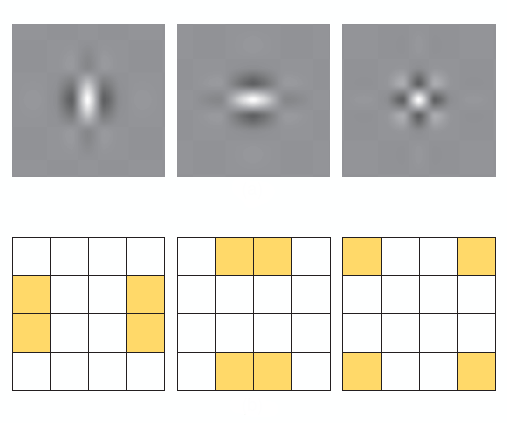
\includegraphics[width=0.5\textwidth]{litreview/images/dwt_wavelets.png}
    \mycaption{Typical wavelets from the 2D separable DWT\@}{Top: Wavelet point
      spread functions for $\psi^v$ (low-high), $\psi^h$ (high-low), and
      $\psi^d$ (high-high) wavelets. High-high wavelets are in a checkerboard
      pattern, with no favoured orientation. Bottom: Idealized support of the
      spectra of each of the wavelets. Image taken from
      \cite{selesnick_dual-tree_2005}.}
      \label{fig:ch2:dwt_wavelets}
  \end{figure}
  % \begin{quote}
    % Always operate at the slowest possible sample rate.
  % \end{quote}

  The 2-D DWT has one scaling fucntion and three wavelet functions, composed of
  the product of 1-D wavelets in the $x$ and $y$ directions:
  \begin{align}
    \phi(x,y) &= \phi(x)\phi(y) \label{eq:ch2:dwt1}\\
    \psi^h(x,y) &= \phi(x) \psi(y) \\
    \psi^v(x,y) & = \psi(x) \phi(y) \\
    \psi^d(x,y) & = \psi(x) \psi(y) \label{eq:ch2:dwt4}
  \end{align}
  with $h, v, d$ indicating the sensitivity to horizontal, vertical and diagonal
  edges. The point spread functions for the wavelet functions are shown in \autoref{fig:ch2:dwt_wavelets}.
  
  \eqref{eq:ch2:2d_shifts} gave the equation for the daughter wavelets in 2-D,
  in 1-D at scales $a=2^j, j \geq 0$, this is simply:
  \begin{equation}
    \psi_{b, j}(x) = 2^{-j/2} \psi\left(\frac{x-b}{2^j} \right)
  \end{equation}
  For the four equations above \eqref{eq:ch2:dwt1} -- \eqref{eq:ch2:dwt4},
  define the daughter wavelets as:
  \begin{equation}
    \psi_{kl}^{\alpha, j}(x,y) = \psi^\alpha_{j,k}(x)\psi^\alpha_{j,l}
  \end{equation}
  for $\alpha = h, v, d,\ k,l \in \integers$. We can then get an orthonormal
  basis with the set $\{ \phi^j_{kl}, \psi^{\alpha,j}_{kl} \}_{\alpha}$.
  The wavelet coefficients at chosen scale and location can then be found by
  taking the inner product of the signal $x$ with the daughter wavelets.

  % A signal $x \in L_2(\reals[2])$ is represented at resolution $2^j$ by the
  % function $x_j = a_j + \sum_\alpha d^\alpha_j$, where:
  % \begin{align}
    % a_j &= \sum_
  % \end{align}

  \subsubsection{Shortcomings}
  The Discrete Wavelet Transform (DWT) is an orthogonal basis. It is a natural
  first signal expansion to consider when frustrated with the limitations of the
  Fourier Transform. It is also a good example of the limitations of
  non-redundant transforms, as it suffers from several drawbacks:
  \begin{itemize}
    \item The DWT is sensitive to the zero crossings of its wavelets. We would
      like singularities in the input to yield large wavelet coefficients, but
      if they fall at a zero crossing of a wavelet, the output can be small. See
      \autoref{fig:ch2:dwt_zero_crossing}.
    \item They have poor directional selectivity. As the wavelets are purely
      real, they have passbands in all four quadrants of the frequency plane.
      While they can pick out edges aligned with the frequency axis, they do
      not have admissibility for other orientations. See
      \autoref{fig:ch2:dwt_wavelets}.
    \item They are not shift invariant. In particular, small shifts greatly
      perturb the wavelet coefficients. \autoref{fig:ch2:dwt_zero_crossing} shows
      this for the centre-left and centre-right images.
      \autoref{fig:ch2:dtcwt_shift_invariance} (right) also shows this.
  \end{itemize}

  The lack of shift invariance and the possibility of low outputs at
  singularities is a price to pay for the critically sampled property of the
  transform. This shortcoming can be overcome with the undecimated DWT
  \cite{mallat_wavelet_1998,coifman_translation-invariant_1995}, 
  but it comes with a heavy computational and memory cost.

  \begin{figure}
    \centering
      \makebox[\textwidth][c]{%
        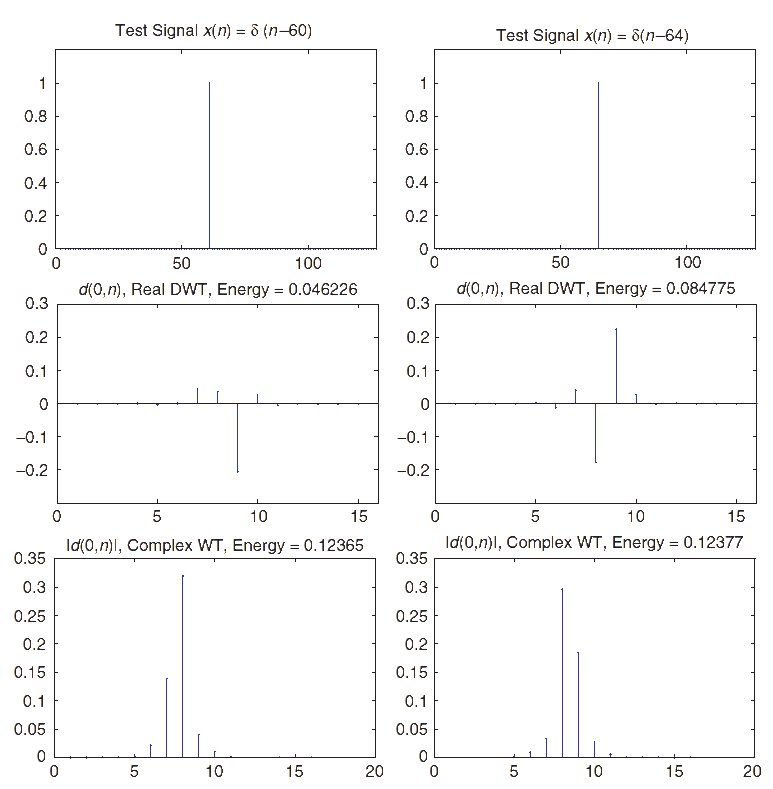
\includegraphics[width=1.1\textwidth]{litreview/images/dwt_zero_crossing.png}
      }
      \mycaption{Sensitivity of DWT coefficients to zero crossings and small
        shifts}{Two impulse signals $\delta(n-60)$ and $\delta(n-64)$ are
        shown (top), as well as the wavelet coefficients for scale $j=1$ for the DWT (middle) and
        for the $\DTCWT$ (bottom). In the middle row, not only are the coefficients very different
        from a shifted input, but the energy has almost doubled. As the DWT is an orthonormal
        transform, this means that this extra energy has come from other scales. In comparison, the
      energy of the magnitude of the $\DTCWT$ coefficients has remained far more constant, as has the
    shape of the envelope of the output.  Image taken from \cite{selesnick_dual-tree_2005}.}
      \label{fig:ch2:dwt_zero_crossing}
  \end{figure}

\subsection{Complex Wavelets}\label{sec:ch2:complex_wavelets}
  Fortunately, we can improve on the DWT with complex wavelets, as they can
  solve these new shortcomings while maintaining the desired localization
  properties. 
  
  The Fourier transform does not suffer from a lack of directional selectivity
  and shift variance, because its basis functions are based on the complex
  sinusoid: 
  \begin{equation} 
    e^{j\omega t} = \cos(\omega t) + j\sin(\omega t)
  \end{equation} 
  whereas the DWT's basis functions are based on only the real
  sinusoid $\cos(\omega t).$\footnote{we have temporarily switched to 1D
  notation here as it is clearer and easier to use, but the results still hold
  for 2D} As $t$ moves along the real line, the phase of the
  Fourier coefficients change linearly, while their magnitude remains constant. In
  contrast, as $t$ moves along the real line, the sign of the real coefficient
  flips between -1 and 1, and its magnitude is a rectified sinusoid.

  These nice properties come from the fact that the cosine and sine functions of the
  Fourier transform form a Hilbert Pair and together constitute an 
  analytic signal.

  We can achieve these nice properties if the mother wavelet for our wavelet
  transform is analytic:
  \begin{equation}
    \psi_{c}(t) = \psi_{r}(t) + j\psi_{c}(t) \label{eq:ch2:complex_wavelet}
  \end{equation}
  where $\psi_{r}(t)$ and $\psi_{c}(t)$ form a Hilbert Pair (i.e.,\ they are
  $90\degs$ out of phase with each other).

  There are a number of possible ways to do a wavelet transform with complex
  wavelets. We examine two in particular, a Fourier-based, sampled CWT using
  Morlet wavelets, and the Dual-Tree Complex Wavelet Transform ($\DTCWT$)
  developed by Kinsbury \cite{kingsbury_wavelet_1997, kingsbury_dual-tree_1998,
  kingsbury_dual-tree_1998-1,  kingsbury_image_1999, kingsbury_shift_1999,
  kingsbury_dual-tree_2000, kingsbury_complex_2001, selesnick_dual-tree_2005}.

  The Morlet wavelet transform we look at as it is used by 
  Mallat et.\ al.\ in their scattering transform
  \cite{bruna_classification_2011, bruna_invariant_2013, bruna_scattering_2013,
  oyallon_generic_2013, oyallon_deep_2015, sifre_rotation_2013,
  sifre_rigid-motion_2014, sifre_rigid-motion_2014-1, sifre_scatnet_2013}, which
  has been a large inspiration for our work, and we will introduce it shortly. 
  The $\DTCWT$ we believe offers
  several advantages over the Morlet based implementation, and has been the
  basis for most of our work.

\subsection{Sampled Morlet Wavelets}\label{sec:ch2:morlet_fourier}
  % Just need to review in Vetterli, how to do FFT based sampling of the CWT.
  The wavelet transform used by Mallat et.\ al.\ in their scattering transform are an efficient
  implementation of the Gabor Transform.  While the Gabor wavelets have the best
  theoretical trade-off between spatial and frequency localization, they have a
  non-zero mean.  This violates \eqref{eq:ch2:admissibility} making them
  inadmissible as wavelets. Instead, the Morlet wavelet has the same shape, but
  with an extra degree of freedom chosen to set $\int \psi (\bmu{u}) d\bmu{u}
  =0$. This wavelet has equation (in 2D):
  \begin{equation}
    \psi(\bmu{u}) = \frac{1}{2\pi\sigma^2} {(e^{i\bmu{u}\xi} - \beta)}
                     e^{-\frac{|\bmu{u}|^2}{2\sigma^2}} 
    \label{eq:ch2:morlet}
  \end{equation}
  where $\beta$ is usually $<<1$ and is this extra degree of freedom, 
  $\sigma$ is the size of the gaussian window, and $\xi$ is the
  location of the peak frequency response --- i.e.,\ for an octave based
  transform, $\xi = 3\pi/4$.

  \citeauthor{bruna_invariant_2013} add an extra degree of freedom in their 
  original design \cite{bruna_invariant_2013} by allowing for a non-circular
  Gaussian window over the complex sinusoid, which gives control over the angular
  resolution of the final wavelet. \eqref{eq:ch2:morlet} now becomes:
  \begin{equation}
    \psi(\bmu{u}) = \frac{\gamma}{2\pi\sigma^2}{(e^{i\bmu{u}\xi} - \beta)}
                  e^{-\bmu{u^t}\Sigma^{-1}  \bmu{u}} 
    \label{eq:ch2:morlet_slant}
  \end{equation}
  Where
  $$\Sigma^{-1} = \left[ \begin{smallmatrix} 
      \frac{1}{2\sigma^2} & 0 \\ 
      0 & \frac{\gamma^2}{2\sigma^2} 
      \end{smallmatrix} \right] $$
  The effects of modifying the eccentricity parameter $\gamma$ and the window size
  $\sigma$ are shown in \autoref{fig:ch2:morlet_filters}. A full family of
  Morlet wavelets at varying scales and orientations is shown in 
  \autoref{fig:ch2:morlet_wavelets_full}.

  % To have a full two
  % dimensional wavelet transform, we need to rotate this mother wavelet by angle
  % $\theta$ and scale it by $j/Q$, where $Q$ is the number of scales per octave
  % (usually 1 in image processing). 

  % This can be done by doing the following
  % substitutions in \eqref{eq:ch2:morlet_slant}:
  % \begin{align*}
    % R_{\theta}& = \left[ \begin{smallmatrix}
                    % \cos(\theta) & -\sin(\theta) \\
                    % \sin(\theta) & \cos(\theta)
                  % \end{smallmatrix} \right] \\
    % \bmu{u}_{\theta} & =  R_{-\theta} \bmu{u} \\
    % \sigma_j & =  2^{\frac{j-1}{Q}} \sigma \\
    % \xi_j & =  \frac{\xi}{2^{\frac{j-1}{Q}}}
  % \end{align*}
  % We can combine these two variables into a single coordinate
  % \begin{equation}
    % \lambda = (\theta, j/Q)
  % \end{equation}
  % We can now scale and rotate this mother wavelet:
  % \begin{equation}
    % \psi_{\lambda}(\bmu{u}) = 2^{-j/Q}\psi(2^{-j/Q}R_{\theta}^{-1} \bmu{u})
  % \end{equation}
  \begin{figure}
    \begin{center}
      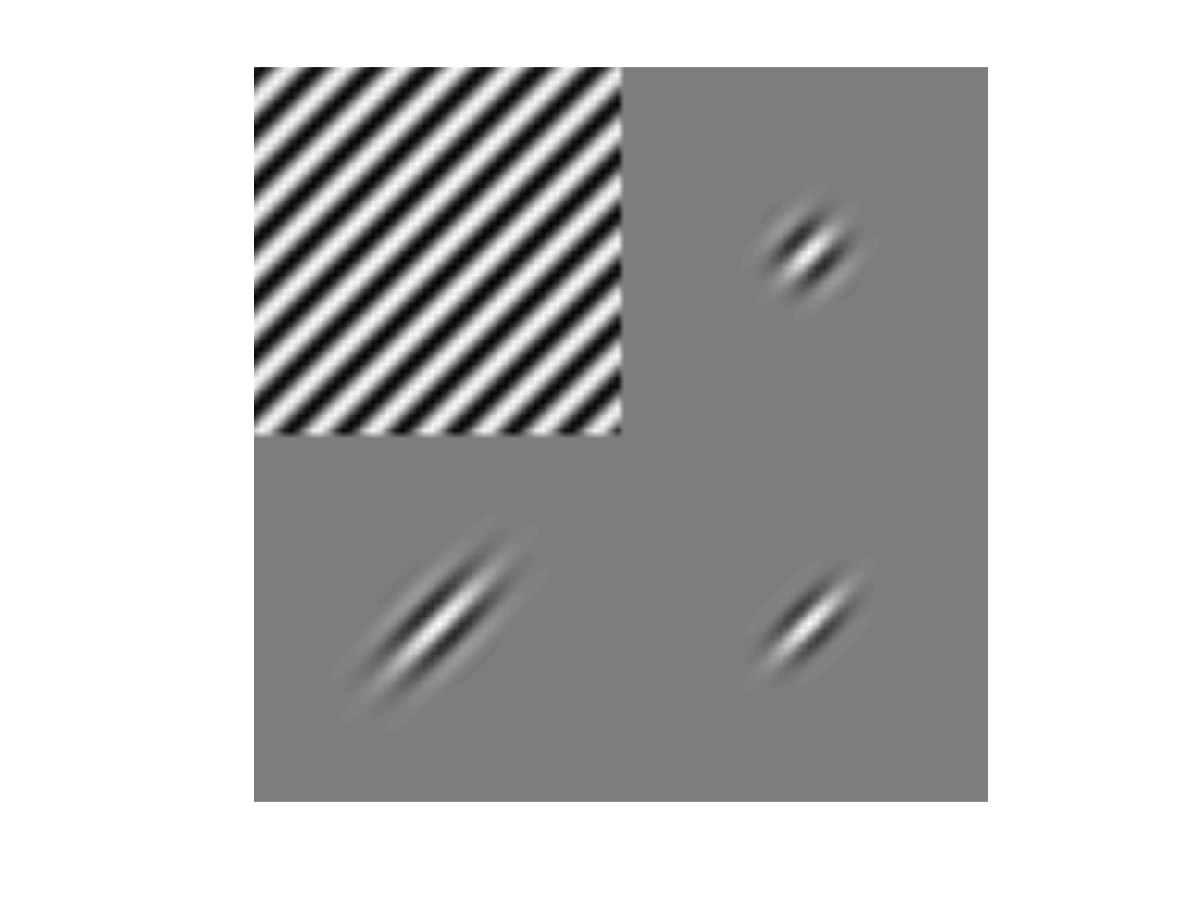
\includegraphics[height=6cm]{\imgpath/morlet_filters.png}
      \mycaption{Single Morlet filter with varying slants and window sizes}
              {Top left --- $45\degs$ plane wave (real part only). Top right --- plane wave with
              $\sigma=3,\gamma=1$. Bottom left --- plane wave with $\sigma=3,\gamma=0.5$. Bottom
            right --- plane wave with $\sigma=2,\gamma=0.5$.}
      \label{fig:ch2:morlet_filters}
    \end{center}
  \end{figure}
  \begin{figure}
    \begin{center}
      \makebox[\textwidth][c]{%
        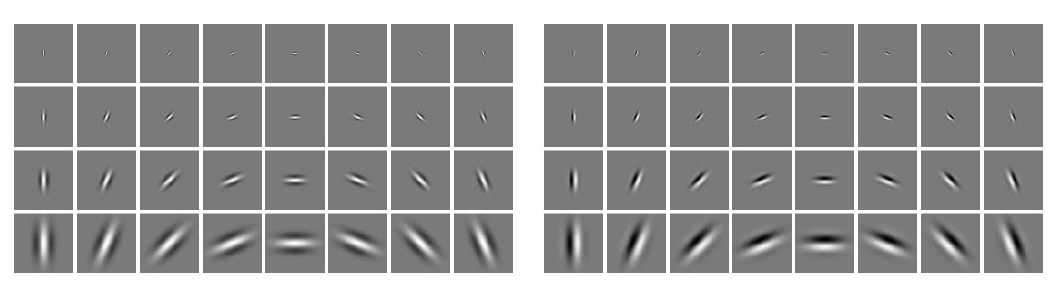
\includegraphics[width=1.1\textwidth]{\imgpath/morlet_wavelets_full.png}
      }
      \mycaption{The full dictionary of Morlet wavelets used by Mallat}
              {The real filters are on the left and the imaginary on the right. The first row
              correspond to scale $j=1$, increasing up to $j=4$. The first column corresponding to
            $\theta = 0$, rotating through $\pi/8$ up to the eighth column of $7\pi/8$,
          $\gamma=1/2$.} 
      \label{fig:ch2:morlet_wavelets_full}
    \end{center}
  \end{figure}

\subsubsection{Invertibility and Energy Conservation}
  We can write the wavelet transform of an input $x$ as 
  \begin{equation}
    \mathcal{W}x = \left\{x \ast \phi_J, x \ast \psi_{\lambda}
    \right\}_{\lambda}
  \end{equation}
  The $\ell^2$ norm of the wavelet transform is then defined by
  \begin{equation}
    \norm{\mathcal{W}x}^2 = \norm{x\ast\phi_J}^2 + \sum_{\lambda}\norm{x \ast
      \psi_\lambda}^2
  \end{equation}
  An energy preserving transform will satisfy Plancherel's equality, so that
  \begin{equation}
    \norm{\mathcal{W}x} = \norm{x}
  \end{equation}
  which is a nice property to have for invertibility, as well as for analysing
  how different signals get transformed (e.g.\ white noise versus standard
  images).
  
  For a transform to be invertible, we examine the measure of how tightly its
  basis functions tile the Fourier plane with its Littlewood-Paley function:  
  \begin{equation}
    A(\omega) = {|\mathcal{F}\phi_J(\omega)|}^2
    + \sum_{\lambda} {|\mathcal{F}\psi_{\lambda}(\omega)|}^2
  \end{equation}
  If the tiling is $\alpha$-tight, then $\forall \omega \in \mathbb{R}^2$:
  \begin{equation}
    1-\alpha \le A(\omega) \le 1
  \end{equation}
  and the wavelet operator, $\mathcal{W}$ is an $\alpha$ frame. If $A(\omega)$
  is ever close to 0, then there is not a good coverage of the frequency plane
  at that location. If it ever exceeds 1, then there is overlap between bases.
  Both of these conditions make invertibility difficult\footnote{In practise,
  if $A(\omega)$ is only slightly greater 1 for only a few small areas of
  $\omega$, approximate inversion can be achieved}.
  \autoref{fig:ch2:morlet_littlewood_paley} show the invertibility of a few
  families of wavelets used by \Mallat. Invertibility is possible, but not
  guaranteed for all configurations. The Fourier transform of the inverse
  filters are defined by:
  \begin{align}
    \mathcal{F}\phi_J^{-1}(\omega) &= A(\omega)^{-1} \mathcal{F}\phi_J(\omega) \\
    \mathcal{F}\psi_{\lambda}^{-1}(\omega) &= A(\omega)^{-1}
      \mathcal{F}\psi_{\lambda}(\omega) 
  \end{align}

  \begin{figure}
    \centering
      \makebox[\textwidth][c]{%
        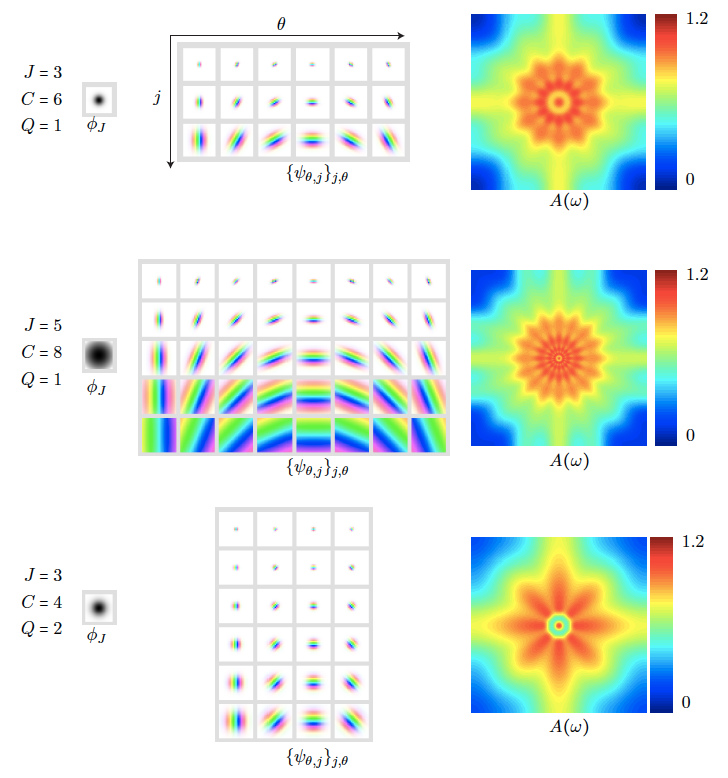
\includegraphics[width=1.1\textwidth]{\imgpath/morlet_littlewood_paley.png}
      }
      \caption[Three Morlet Wavelet Families and their tiling of the frequency
              plane]
              {Three Morlet Wavelet Families and their tiling of the frequency
              plane. For each set of parameters, the point spread functions of
              the wavelet bases are shown, next to their Littlewood-Paley sum
              $A(\omega)$. None of the configurations cover the corners of the
              frequency plane, and they often exceed 1. 
              Increasing $J$, $L$ (Sifre uses $C$ in these
              diagrams) or $Q$ gives better frequency localization but at the
              cost of spatial localization and added complexity. Image taken
              from \cite{sifre_rigid-motion_2014-1}.}
      \label{fig:ch2:morlet_littlewood_paley}
  \end{figure}


% The discrete wavelet transform (DWT) provides a non-redundant representation
  % of

% signals, hence overcomes the problem of redundancy. The DWT samples the
% timefrequency
% plane and only preserves the least number of the discrete coefficients
% that are required for perfect synthesis. The scale parameter a is sampled first
% on a logarithmic grid, and then the time parameter b is sampled with respect to
% the scale parameter. Though any sampling rate is possible, the DWT is mostly
% computed on the dyadic grid such that the DWT can be efficiently implemented
% by filter bank trees. This is of real value for practical applications.
% Figure 3.1 shows the diagram for a 4-level forward and inverse DWT, which
% explains how the DWT can be efficiently implemented by octave-band,
% discretetime
% filter bank trees. The notations in the diagram have the following meanings:
% 1. x is the original signal
% 2. ˆx is the reconstructed signal
% 3. H0 is the low-pass decomposition filter
% 4. H1 is the high-pass decomposition filter
% 5. °#2 is the operation that downsamples the signal by 2
% 6. G0 is the low-pass reconstruction filter
% 7. G1 is the high-pass reconstruction filter
% 8. °"2 is the operation that upsamples the signal by 2 by inserting zeros
% 9. w(j) are the wavelet coefficients in the j-th subband.
% The decomposition filter (H0, H1) and reconstruction filters (G0, G1) are
% carefully
% chosen in order that the wavelet transform can be inverted, i.e. x = ˆx. The
% above procedure can be represented by matrix-vector notations, which will later
% be introduced in 3.2.3.
% 
\subsection{The $\DTCWT$}
  The $\DTCWT$ was first proposed by \citeauthor{kingsbury_dual-tree_1998} in
  \cite{kingsbury_dual-tree_1998, kingsbury_dual-tree_1998-1} as a way to combat
  many of the shortcomings of the DWT, in particular, its poor directional
  selectivity, and its poor shift invariance. A thorough analsysis of the
  properties and benefits of the $\DTCWT$ is done in
  \cite{kingsbury_image_1999,selesnick_dual-tree_2005}. Building on these
  properties, it been used
  successfully for denoising and inverse problems \cite{rivaz_bayesian_2001,
  zhang_bayesian_2008, zhang_variational_2015, miller_image_2008}, texture
  classification \cite{hatipoglu_texture_1999, rivaz_complex_1999}, image
  registration \cite{loo_motion-estimation-based_2001, chen_efficient_2012}
  and
  SIFT-style keypoint generation matching \cite{fauqueur_multiscale_2006,
  anderson_determining_2005, anderson_rotation-invariant_2006,
  bendale_multiscale_2010, ng_robust_2012} amongst many other applications. 

  Compared to Gabor (or Morlet) image analysis, the authors of
  \cite{selesnick_dual-tree_2005} sum up the dangers as:
  \begin{quote}
    A typical Gabor image analysis is either expensive to compute, is
    noninvertible, or both.
  \end{quote}
  This nicely summarises the difference between this method and the Fourier
  based method outlined in \autoref{sec:ch2:morlet_fourier}. The $\DTCWT$ is
  a filter bank (FB) based wavelet transform. It is faster
  to implement than the Morlet analysis, as well as being more readily invertible.

\subsubsection{Deisgn Criteria for the $\DTCWT$}
  It was stated in
  \autoref{sec:ch2:complex_wavelets} that if the mother (and daughter) wavelets
  were complex, with their real and imaginary parts forming a Hilbert pair,
  then the wavelet transform of a signal with these $\{\psi_{j,n}\}_{j,n}$
  would give a representation that had nice shift properties\footnote{in
  particular, that a shift in input gives the same shift in magnitude of the
  wavelet coefficients, and a linear phase shift}, was insensitive to zero crossings of the
  wavelet, and had good directional selectivity. 
  
  As in \autoref{sec:ch2:complex_wavelets}, we want to have a complex mother
  wavelet $\psi_c$ that satisfies \eqref{eq:ch2:complex_wavelet}, but now
  achieved with filter banks. A slight deviation from standard filter bank
  notation, where $h_0, h_1$ are the analysis and $g_0,g_1$ are the synthesis
  filters. We define:
  \begin{itemize}
    \item $h_0, h_1$ the low and high-pass analysis filters for $\psi_r$ (henceforth called
      $\psi_h$)
    \item $g_0, g_1$ the low and high-pass analysis fitlers for $\psi_i$
      (henceforth called $\psi_g$)
    \item $\tilde{h}_0, \tilde{h}_1$ the low and high-pass synthesis filters
      for $\tilde{\psi}_h$.
    \item $\tilde{g}_0, \tilde{g}_1$ the low and hig pass synthesis filters for
      $\tilde{\psi}_g$.
  \end{itemize}

  The dilation and wavelet equations for a 1D filter bank implementation are:
  \begin{align}
    \phi_h(t) & =  \sqrt{2} \sum_n h_0(n) \phi_h(2t-n) \\
    \psi_h(t) & =  \sqrt{2} \sum_n h_1(n) \phi_h(2t-n) \\
    \phi_g(t) & =  \sqrt{2} \sum_n g_0(n) \phi_g(2t-n) \\
    \psi_g(t) & =  \sqrt{2} \sum_n g_1(n) \phi_g(2t-n) 
  \end{align}
  This implementation is shown in \autoref{fig:ch2:dtcwt_1d_fb}.

  \begin{figure}
    \centering
      % 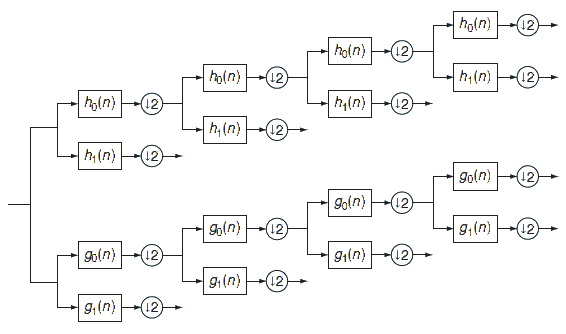
\includegraphics[width=\textwidth]{images/dtcwt_1d_fb.png}
      \caption[Analysis FB for the $\DTCWT$]
              {Analysis FB for the $\DTCWT$@. Top `tree' forms the real
              component of the complex wavelet $\psi_r$, and the bottom tree forms the
              imaginary (Hilbert pair) component $\psi_i$. Image taken from
              \cite{selesnick_dual-tree_2005}.}
      \label{fig:ch2:dtcwt_1d_fb}
  \end{figure}

  Designing a filter bank implementation that results in Hilbert symmetric
  wavelets does not appear to be an easy task. However, it was shown
  by \citeauthor{kingsbury_image_1999} in \cite{kingsbury_image_1999} (and later proved by
  \citeauthor{selesnick_hilbert_2001} in \cite{selesnick_hilbert_2001}) that the
  necessary conditions are conceptually very simple. One low-pass filter must be
  a \emph{half-sample shift} of the other. I.e.,\ 
  \begin{equation}
    g_0(n) \approx h_0(n-0.5) \rightarrow \psi_g(t) \approx
    \mathcal{H}\{\psi_h(t)\}
  \end{equation}
  As the $\DTCWT$ is designed as an invertible filter bank implementation, this
  is only one of the constraints. Naturally, there are also:
  \begin{itemize}
    \item Perfect reconstruction
    \item Finite support
    \item Linear phase
    \item Many vanishing moments at $z=-1$ for good stopband properties
  \end{itemize}
  to consider when building the $h$'s and $g$'s.
  The derivation of the filters that meet these conditions is covered in
  detail in \cite{kingsbury_complex_2001, kingsbury_design_2003}, and in
  general in \cite{selesnick_dual-tree_2005}. The result is the
  option of three families of filters:  biorthogonal filters ($h_0[n] =
  h_0[N-1-n]$ and $g_0[n] = g_0[N-n]$), q-shift filters ($g_0[n]
  = h_0[N-1-n]$), and common-factor filters.

\subsubsection{The Resulting Wavelets and their Properties}
  While analytic wavelets in 1D are useful for their shift invariance, the real
  beauty of the $\DTCWT$ is in its ability to make a separable 2D wavelet
  transform with oriented wavelets. 
  
  \autoref{fig:ch2:dwt_hh} shows the spectrum of
  the wavelet when the separable product uses purely real wavelets, as is the
  case with the DWT\@. \autoref{fig:ch2:dtcwt_hh} however, shows the separable
  product of two complex, analytic wavelets resulting in a localized and
  oriented 2D wavelet.  
  
  I.e.,\ for the $+45\degs$ wavelet\footnote{note that \autoref{fig:ch2:dtcwt_hh}
  shows the $135\degs$ wavelet} (which is high
  in both $\omega_1$ and $\omega_2$), the separable product is:
  \begin{align}
    \psi(\omega_1,\omega_2) & =  \psi_c (\omega_1) \overline{\psi_c
      (\omega_2) } \label{eq:ch2:wavelet_separable_product}\\
    & =  (\psi_h(\omega_1) + j \psi_g(\omega_1) \overline{\left(\psi_h(\omega_2)
      + \psi_g(\omega_2) \right)} \nonumber\\
    & =  \psi_h(\omega_1) \psi_h(\omega_2) + \psi_g(\omega_1)
      \psi_g(\omega_2)\nonumber\\
    &  + j\left( \psi_g(\omega_1) \psi_h(\omega_2) - \psi_h(\omega_1)
        \psi_g(\omega_2) \right)  \label{eq:ch2:dtcwt_2d_product}
  \end{align}
  Similar equations can be obtained for the other five wavelets and the scaling
  function, by replacing
  $\psi$ with $\phi$ for both directions, and not taking the complex conjugate
  in \eqref{eq:ch2:wavelet_separable_product} to get the right hand side of the
  frequency plane. 
  
  \autoref{fig:ch2:dtcwt_wavelets} shows the resulting wavelets both in the spatial
  domain and their idealized support in the frequency domain.

  \autoref{fig:ch2:dtcwt_shift_invariance} shows how the $\DTCWT$ compares with the
  DWT with a shifting input.

  \begin{figure}
%      \centering
      \subfloat[]{\makebox[\textwidth][c]{%
        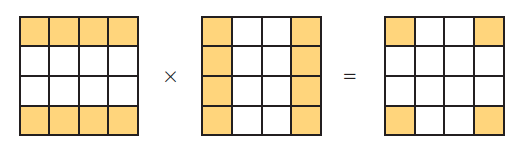
\includegraphics[width=0.8\textwidth]{\imgpath/dwt_hh.png}
        \label{fig:ch2:dwt_hh}}}
      \newline
      \subfloat[]{\makebox[\textwidth][c]{%
        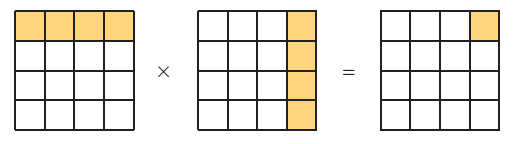
\includegraphics[width=0.8\textwidth]{\imgpath/dtcwt_hh.png}
        \label{fig:ch2:dtcwt_hh}}}
      \caption[The DWT high-high vs the $\DTCWT$ high-high frequency support]
              {\subref{fig:ch2:dwt_hh} The high-high DWT wavelet having a passband in
              all 4 corners of the frequency plane vs \subref{fig:ch2:dtcwt_hh} the
              high-high $\DTCWT$ wavelet frequency support only existing in one
              quadrant. Taken from \cite{selesnick_dual-tree_2005}}
      \label{fig:ch2:dwt_dtcwt_hh}
  \end{figure}

  \begin{figure}
    \centering
      % 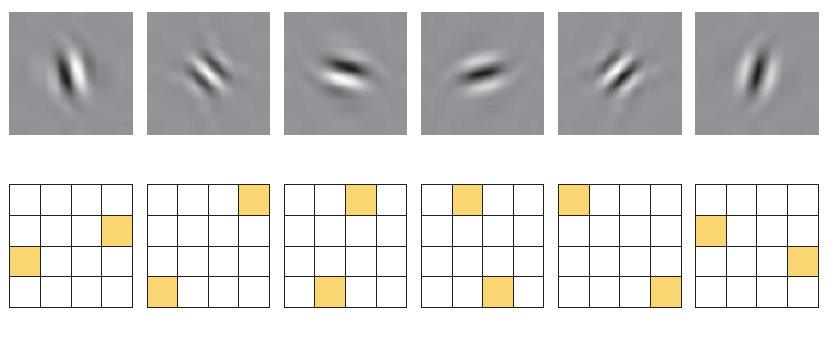
\includegraphics[width=\textwidth]{images/dtcwt_wavelets.png}
      \caption[Wavelets from the 2D $\DTCWT$]
              {Wavelets from the 2d $\DTCWT$@. \textbf{Top:} The six  oriented filters
      in the space domain (only the real wavelets are shown). \textbf{Bottom:}
      Idealized support of the Fourier spectrum of each wavelet in the 2D
      frequency plane. Spectra of the the real wavelets are shown --- the
      spectra of the complex wavelets ($\psi_h + j\psi_g$) only has support in the top
      half of the plane. Image taken from \cite{selesnick_dual-tree_2005}.}
      \label{fig:ch2:dtcwt_wavelets}
  \end{figure}
  \begin{figure}
    \centering
      \makebox[\textwidth][c]{%
        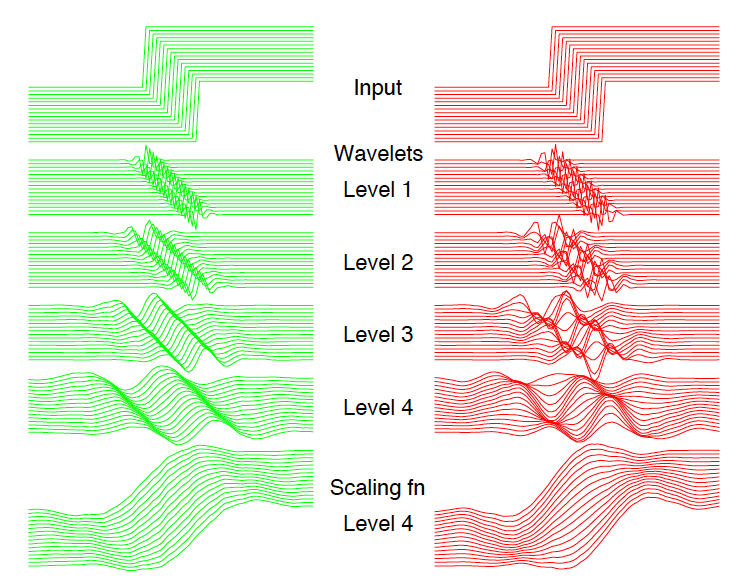
\includegraphics[width=1.1\textwidth]{\imgpath/dtcwt_shift_invariance.png}
      }
      \mycaption{The shift invariance ofthe $\DTCWT$ vs.\ the real DWT}
        {The $\DTCWT$ (left) linearizes shifts in the phase change of the complex
        wavelet. The DWT (right) cannot do this and suffers from shift variance. 
        Image taken from \cite{kingsbury_dual-tree_1998}.}
      \label{fig:ch2:dtcwt_shift_invariance}
  \end{figure}

  
\subsubsection{Invertibility and Energy Conservation}
  We analysed the Littlewood-Paley function for the Morlet-Fourier
  implementation, and saw what areas of the spectrum were better covered than
  others. How about for the $\DTCWT$?

  It is important to note that in the case of the $\DTCWT$, the wavelet
  transform is also approximately unitary, i.e.,\
  \begin{equation}
    \norm{x}^2 \approx \norm{\mathcal{W}x}^2
  \end{equation}
  and the implementation is perfectly invertible as the Littlewood-Paley
  function is unity (or very near unity) $\forall \omega$. See
  \autoref{fig:ch2:dtcwt_lwoodpaley}. This is not a surprise, as it is a design
  constraint in choosing the filters, but nonetheless is important to note. 

  A beneficial property of energy conservation is that the noise in the input
  will equal the noise in the wavelet coefficients. When we introduce
  Scatternets, we can show that we can keep the unitary property in the
  scattering coefficients. This is an important property, particularly in light
  of the recent investigations in \cite{szegedy_intriguing_2013}. This paper
  saw that it is easy to find cases in CNNs where a small amount of input
  perturbation results in a completely different class label (see
  \autoref{fig:ch2:difference}). Having a unitary transform limits the
  amount the features can change, which will make the entire network more
  stable to distortion and noise.

  \begin{figure}
    \subfloat{\makebox[0.6\textwidth][c]{%
      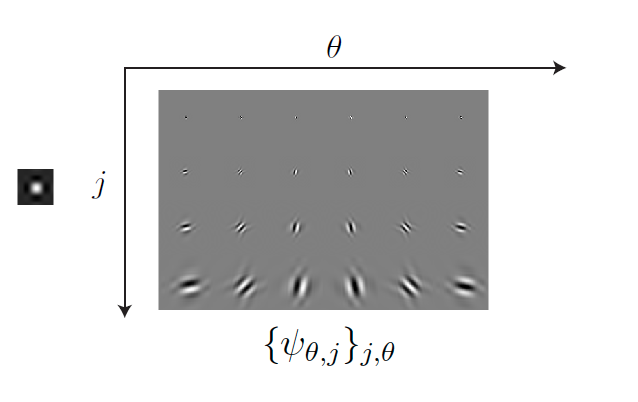
\includegraphics[width=0.7\textwidth,valign=c]{\imgpath/dtcwt_real_4scales.png}
    }}
    \subfloat{\makebox[0.4\textwidth][c]{%
      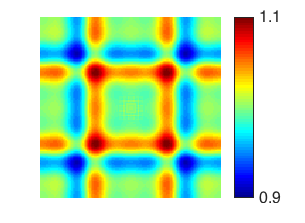
\includegraphics[width=0.5\textwidth,valign=c]{\imgpath/dtcwt_lwoodpaley_2.png}
    }}
    \caption[$\DTCWT$ basis functions and their frequency coverage]
    {Four scales of the $\DTCWT$ (left) and its associated frequency
    coverage, or $A(\omega)$ (right). Note the reduced scale compared to \autoref{fig:ch2:morlet_littlewood_paley}.}
    \label{fig:ch2:dtcwt_lwoodpaley}
  \end{figure}

  \begin{figure}
    \centering
    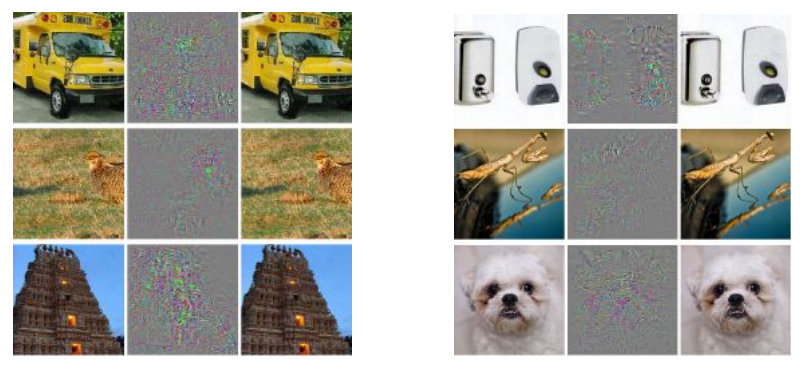
\includegraphics[width=0.9\textwidth]{\imgpath/adversarial_nets.png}
    \mycaption
    {Two adversarial examples generated for AlexNet}{The left column
    shows a correctly predicted sample, the right column an incorrectly
    predicted example, and the centre column the difference between the two
    images, magnified 10 times. Image taken from
    \cite{szegedy_intriguing_2013}.}
    \label{fig:ch2:difference}
  \end{figure}
\subsection{Summary of Methods}
  One final comparison to make between the $\DTCWT$ and the Morlet wavelets is
  their frequency coverage. The Morlet wavelets can be made to be tighter than
  the $\DTCWT$, which gives better angular resolution --- see
  \autoref{fig:ch2:wavelet_freq_resp}. However it is not always
  better to keep getting finer and finer resolutions, indeed the Fourier
  transform gives the ultimate in angular resolution, but as mentioned, this
  makes it less stable to shifts and deformations. 

  \autoref{tab:dtcwt_vs_dwt_vs_mallat} compares the advantages and
  disadvantages of the wavelet methods discussed in this chapter.

  \begin{figure}
    \subfloat[$\DTCWT$ wavelets (left to right) --- $15\degs$, $45\degs$ and $75\degs$]{%
      \makebox[\textwidth][c]{%
      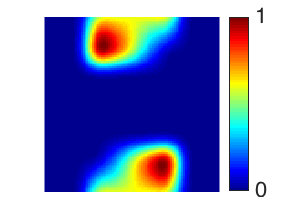
\includegraphics[width=0.4\textwidth]{\imgpath/dtcwt_15deg_energy.png}
      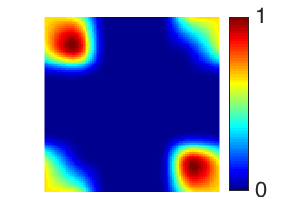
\includegraphics[width=0.4\textwidth]{\imgpath/dtcwt_45deg_energy.png}
      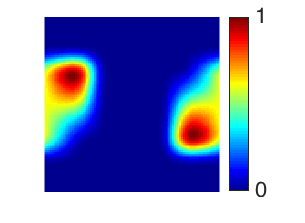
\includegraphics[width=0.4\textwidth]{\imgpath/dtcwt_75deg_energy.png}
    }}
    \newline
    \subfloat{%
      \makebox[\textwidth][c]{%
      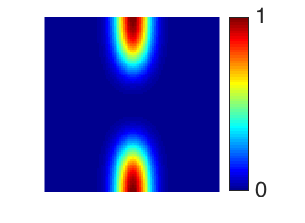
\includegraphics[width=0.4\textwidth]{\imgpath/mallat_0deg_energy.png}
      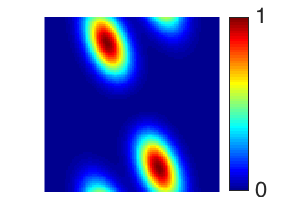
\includegraphics[width=0.4\textwidth]{\imgpath/mallat_225deg_energy.png}
      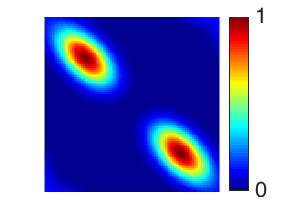
\includegraphics[width=0.4\textwidth]{\imgpath/mallat_45deg_energy.png}
    }}
    \newline
    \subfloat[Morlet wavelets (left to right) --- $0\degs$, $22.5\degs$, $45\degs$, 
              $67.5\degs$,  and $90\degs$]{%
      % Use two makebox commands to center the images
      \makebox[0.5\textwidth][c]{%
        \hspace{1cm}
        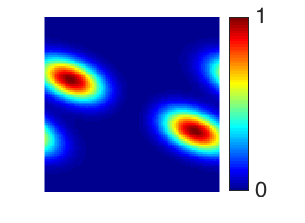
\includegraphics[width=0.4\textwidth,center]{\imgpath/mallat_675deg_energy.png}
      }
      \makebox[0.5\textwidth][c]{%
        \hspace{-1cm}
        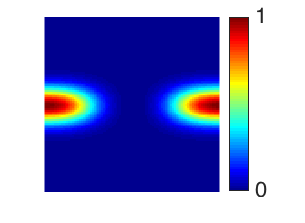
\includegraphics[width=0.4\textwidth,center]{\imgpath/mallat_90deg_energy.png}
      }
    }
    \caption[Comparison of the energy spectra for $\DTCWT$ wavelets to Morlet
    wavelets]
    {Normalized Energy spectra of the $\DTCWT$ wavelets versus the preferred
            8 orientation Morlet wavelets by Mallat for the second quadrant.
            Orientations listed refer to the edge orientation in the spatial
            domain that gives the highest response. All wavelets have been
            normalized to be between zero and one.
            The Morlet wavelets have finer angular
            resolution, which can give better discrimination, at the cost of
            decreasing stability to deformations, and requiring larger spatial
            support.}
    \label{fig:ch2:wavelet_freq_resp}
  \end{figure}
